\subsubsection{Batalimo-Maluba-Gruppe}\label{sec:BTM-Gr}

Das bisher älteste, hinreichend sicher datierte keramische Material aus dem nördlichen Bereich des Arbeitsgebietes entlang des mittleren \mbox{Ubangi} ist durch die Batalimo-Maluba-Gruppe repräsentiert. Sie gründet im Kern auf den keramischen Inventaren der Fundstellen Batalimo am Lobaye (Abb.~\ref{fig:BTM-Verbreitung}), in der südwestlichen Zentralafrikanischen Republik gelegen, und Maluba am Lua (Fpl.~230). Die Fundstelle in Batalimo wurde 1966 im Rahmen von Baumaßnahmen entdeckt \parencite[206\,f.]{deBayledesHermens.1975}. Bei Erdarbeiten zur Errichtung eines Heizöltanks wurde unter anderem ein Steinbeil gefunden. Roger de Bayle des Hermens besichtigte 1967 die Fundstelle und führte 1968 nahe des Heizöltanks eine kleine Grabung durch, bei der sechs zusammenhängende Ein-Meter-Quadranten, zusammen eine 2\,$\times$\,3\,m große Fläche, untersucht wurden.\footnote{Unter der Wurzelzone und einer etwa 0,45\,m mächtigen, sterilen Sand-Schicht wurde eine zwischen 0,1--0,7\,m mächtige Kultur-Schicht freigelegt, welche viel Silex und Keramik erbrachte (\textsc{de Bayle des Hermens} 1975: 206\,f., Taf.~32). Die Grabungen erbrachten ein Silex-Inventar aus 6824 Abschlägne und 287 Werkzeugformen, einschließlich einer größeren Anzahl geschlagener sowie teilweise polierter beziehungsweise geschliffener Beilformen (ebd. 214--219 Abb.~99--101). Das keramische Material der Grabung in Batalimo umfasst neben drei fast vollständig erhaltenen Gefäßen auch 922 Scherben, welche sich zu 32 Gefäßeinheiten zusammenfassen ließen \parencite[221--234, Taf.~33--34]{Aumassip.1975}. Die Keramik aus Batalimo wies einen hohen Zerscherbungsgrad auf, so waren mehr als 50\,\% des Materials kleiner als 1\,cm\textsuperscript{2} und nur etwas mehr als 10\,\% größer als 25\,cm\textsuperscript{2}.} Diese Grabungen deuteten für Jahrzehnte eine enge Assoziierung von Steingeräten und Keramik an, da vom Ausgräber eine Vermischung der Inventare ausgeschlossen wurde \parencites[211\,f.]{deBayledesHermens.1975}[nach][137]{Eggert.1987c}.

Im Jahr 1981 öffnete Pierre Vidal eine 1\,m\textsuperscript{2} große Sondagefläche an der Fundstelle \parencite[43]{Kote.1992}\footnote{Weder zu Befunden noch Funden, die im Zuge dieser Maßnahme angetroffen wurden, liegen dezidierte Angaben vor. Lediglich eine Radiokohlenstoffdatierung ist überliefert. Diese datiert in das 3.--7.~Jh.~n.~Chr (Gif-5894).} und zwischen 1987 und 1990 wurden fünf weitere Grabungsflächen durch eine Arbeitsgruppe um Lassina \textsc{Koté} (ebd.~43, 68 Abb.~9) archäologisch untersucht. Die nach \textcite[207, 209--210 Abb.~93--97]{deBayledesHermens.1975} zwischen 0,1--0,7\,m mächtige dunkle \textit{Kulturschicht} konnte auch von \textcite[66]{Kote.1992} beobachtet werden, wenngleich sie in den jüngeren Grabungen nur zwischen 0,1--0,45\,m mächtig war.\footnote{Den einzelnen Grabungsflächen wurden Kennungen von Z\,III bis Z\,VII gegeben (\textsc{Koté} 1992: 68 Abb.~9). Die 1967 durch \textcite{deBayledesHermens.1975} durchgeführte Grabung wurde als Z\,I und der 1981 durch Vidal angelegte Sondagekasten als Z\,II in die Benennung integriert \parencite[117\,f. Tab.~10]{Kote.1992}. Die Grabungsfläche Z\,IV von Koté schließt dabei an den 1981 durch Vidal geöffneten 1\,m\textsuperscript{2} großen Sondagekasten Z\,II an (ebd. 122). In Schnitt Z\,IV konnten vier fundreiche \textit{Kulturschichten} erfasst werden. Die Funddichte innerhalb der oberen drei Schichten des 28\,m\textsuperscript{2} großen Schnitts lag zwischen 1--1,4\,kg/m\textsuperscript{3} (ebd. 75 Tab.~2). Die unterste, vierte Schicht wies eine Funddichte von lediglich 0,2\,kg/m\textsuperscript{3} auf. Die Funddichte in Schnitt Z\,VI, der 12\,m\textsuperscript{2} groß war und in dem fünf fundführende Schichten erkannt wurden, variierte deutlich. In den oberen beiden Schichten lag sie zwischen 2--3\,kg/m\textsuperscript{3}, die mittlere dritte Schicht wies eine Funddichte von knapp 8\,kg/m\textsuperscript{3} auf, während die darunter liegenden Schichten lediglich zwischen 0,3--0,4\,kg/m\textsuperscript{3} keramische Funde enthielten (ebd.~78 Tab.~3). Zum Vergleich, die Funddichte innerhalb der Grube MLB~85/1-3-1 lag bei zirka 5\,kg/m\textsuperscript{3} (Kat.-Nr.~1).} Weitere archäologische Befunde aus den Grabungen umfassen je eine Grube in Schnitt Z\,III (ebd. 71 Abb.~11--12)\footnote{Leider waren die Grabungsfotografien in der vorliegenden Mikrofiche-Kopie der Arbeit von \textsc{Koté} (1992) aufgrund des Reproduziervorgangs vollkommen unkenntlich, so dass sie als Quellen nicht verwendet werden konnten.} und Z\,VI sowie eine Konzentration großer Keramikfragmente in Schnitt Z\,VI (ebd. 70). Im Schnitt Z\,IV wurde eine kleine Grube, eine durch eine feste Schicht überdeckte Konzentration aus Silexabschlägen und ein einzelnes Gefäß entdeckt (ebd. 71 Abb.~11--12). Die Grabungen haben keramisches Material erfasst, welches eindeutig der Batalimo-Maluba-Grupppe zugerechnet werden kann (ebd. 183--187 Abb.~60--64).\footnote{Die von \textsc{Koté} (1992) vorgelegte Analyse der Materialien behandelt die Funde summarisch und lässt keine Rückschlüsse zu, welche der abgebildeten Formen (ebd. 183--187 Abb.~60--64) zu welchem spezifischen stratigraphischen Kontext gehören. Da sich auch der Bezug zwischen Grabungsbefunden und Radiokohlenstoffdatierungen nur in groben Zügen nachvollziehen ließ, kann nicht mehr abgeleitet werden, welche stratigraphische Einheit sich durch welches Fundspektrum auszeichnete und durch welchen absoluten Datierungsansatz sie zeitlich eingeordnet werden kann.\label{ftn:Kote1992ZuordnungProblem}}

Im Zuge jüngerer Nachgrabungen in Batalimo durch \textcite{Ndanga.2010} wurde deutlich, dass die 1968 von de Bayle des Hermens beobachte Assoziation der Keramik der Batalimo-Maluba-Gruppe mit teilweise polierten Steinartefakten nicht aufrecht erhalten werden kann.\footnote{Im Bereich der ursprünglichen Fundstelle untersuchte Gruben enthielten keine Steinartefakte. Mehrere Testschnitte in einiger Entfernung von der ursprünglichen, nah am Lobaye-Fluss gelgenen Fundstelle ergaben, dass sich die 1968 beobachtete, Steinartefakte und Keramik enthaltende Schicht, in zwei getrennte Schichten aufteilt. Die untere zeichnete sich durch die lithische Industrie aus, während die obere Keramik der Batalimo-Maluba-Gruppe enthielt (mündl. Mitt. E.~Cornelissen 2014). Im Oktober 2014 bot sich die Möglichkeit, die 2010 in Batalimo ausgegrabene Keramik in Augenschein zu nehmen, die sich zu diesem Zeitpunk für erste Restaurierungsarbeiten im \textit{Musée royal de l’Afrique centrale} in Tervuren (Belgien) befand. Das Material zeigte keine auffälligen Unterschiede zu den im Rahmen dieser Arbeit bearbeiteten Funden aus Maluba am Lua (Fpl.~230) oder anderen Fundstellen mit entsprechender Keramik. Auch der relativ starke Grad der Fragmentierung der Stücke schien mit den hier beschriebenen Komplexen vergleichbar. Die an diesem neuen Material beobachteten technologischen Eigenschaften der Scherben entsprechen ebenfalls dem aus dem \mbox{Ubangi}-Gebiet bekannten Spektrum. Lediglich zwei Scherben fielen heraus, beide sind potenziell der \mbox{Ngbanja}-Gruppe zugehörig (siehe Kap.~ \ref{sec:NGB-Gr}).} Leider liegt zum gegenwärtigen Zeitpunkt keine dezidierte Auswertung dieser Grabung vor. Die kommunizierten Ergebnisse unterstützen jedoch die Beobachtungen Eggerts in Maluba (Fpl.~230) sowie an anderen Fundstellen, an denen Batalimo-Maluba-Keramik nie mit Steinartefakten assoziiert gefunden werden konnte. Bereits in seiner ersten Publikation der Ergebnisse der Feldarbeit von 1985 entlang des \mbox{Ubangi} legt \textcite[137]{Eggert.1987c} seine Zweifel am Postulat einer Assoziation der Batalimo-Maluba-Keramik mit teilweise geschliffenen Steinbeilen durch \textcite[212f.]{deBayledesHermens.1975} dar.

Die Fundstelle in Maluba (Fpl.~230) wurden bei der Prospektion entlang des Lua durch das \textit{River Reconnaissance Project} im Jahr 1985 entdeckt. Im Anschluss an die Befahrung des Lua bis nach Fulu-Kaba (Fpl.~233) wurden Grabungen in Maluba durchgeführt, wobei unter anderem zwei Gruben mit der aus Batalimo bekannten Keramik erfasst werden konnten (Kat.-Nr.~1--2). Des Weiteren wurden zwei mutmaßlich subrezente Gruben dokumentiert (Kat.-Nr.~4--5). Bereits im Gelände wurde die starke stilistische Übereinstimmung der Keramik aus den beiden erst genannten Gruben in Maluba (Kat.-Nr.~1--2) zu dem aus Batalimo bekannten Material \parencite[Taf.~33--34]{Aumassip.1975} deutlich. Aufgrund dieser Beobachtung wurde das formale Spektrum des Fundgutes von \textcite{Eggert.1987c} unter dem Terminus \enquote{Batalimo-Maluba-Gruppe} subsumiert beschrieben.

Die Prospektion des \textit{River Reconnaissance Project} entlang des \mbox{Ubangi} im Jahr 1985 erbrachte Batalimo-Maluba-Keramik an 18 verschiedenen Fundstellen. Diese liegen mit Ausnahme des am Lua gelegenen Maluba (Fpl.~230) sämtlich am mittleren und oberen \mbox{Ubangi}, wobei \mbox{Ngbanja} (Fpl.~199) die südlichste und Mokelo (Fpl.~213) die nördlichste Fundstelle des Verbreitungsgebietes ist (Abb.~\ref{fig:BTM-Verbreitung}). Insgesamt konnten 226 GE beziehungsweise 13\,kg Gefäßkeramik der Stilgruppe zugerechnet werden. Eine großer Teil, genauer etwa 63\,\% des Fundgutes, stammt aus den Grabungen in Maluba am Lua (Fpl.~230). Die Funde aus den Oberflächenabsammlungen (37\,\%) umfassen, mit Ausnahme der Fundplätze Dongo (28~GE, Fpl.~202), Mokelo (20~GE, Fpl.~213) und Nzambi (14~GE, Fpl.~205), nur sehr wenige GE je Fundplatz.

\paragraph{Technologische Merkmale}\hspace{-.5em}|\hspace{.5em}%
Die Keramik der Batalimo-Maluba-Gruppe zeichnet sich durch Scherben mit deutlich sichtbaren nichtplastischen Partikeln aus. Alle GE zeigen mindestens einen mittelhohen Anteil nichtplastischer Partikel (7--10\,\%) und 55\,\% weisen einen sehr hohen Anteil auf (25--40\,\%). Vornehmlich bestehen diese aus Mischungen heterogener Quarzsande, aber auch möglicherweise zerstoßene Laterit-Stücke oder andere rötliche Gesteine sowie Organik konnten beobachtet werden. War eine Ansprache der Brennfarbe der verwandten Tone möglich, so ließen sich häufig (47\,\%) rotbrennende Tone beobachten. Nur zu einem geringen Anteil (9\,\%) liegen Hinweise für die Nutzung weißbrennender Tone vor. Innerhalb der Gruppe der nicht klar ansprechbaren Stücke dominieren schwarz, grau, beige sowie braun gefärbte Scherben. Die Batalimo-Maluba-Keramik ist durch die \textit{Fabrics} 5a (35\,\%), 4a (26\,\%), 5b (15\,\%) sowie 4c (10\,\%) bestimmt, die sich neben ihren hohen Anteilen nichtplastischer Partikel durch eine rote Brennfarbe sowie das Fehlen ausgeprägter farblicher Grenzen im Bruch auszeichnen. Die Oberflächen der Stücke sind gleichermaßen rau (31\,\%), leicht rau (30\,\%) oder glatt (29\,\%). Raue Oberflächen sind in vielen Fällen jedoch auf Erosion zurückführbar. Gerade die aufwendig verzierten Stücke (siehe Abb.~\ref{Fig-BatMLB-Typvertreter}) zeigen stark geglättete Oberflächen. Die Wandungsdicke der Stücke liegt im Mittel bei knapp 7\,mm und schwankt zwischen 3--12\,mm.

\begin{figure*}[!tb]
	\centering
	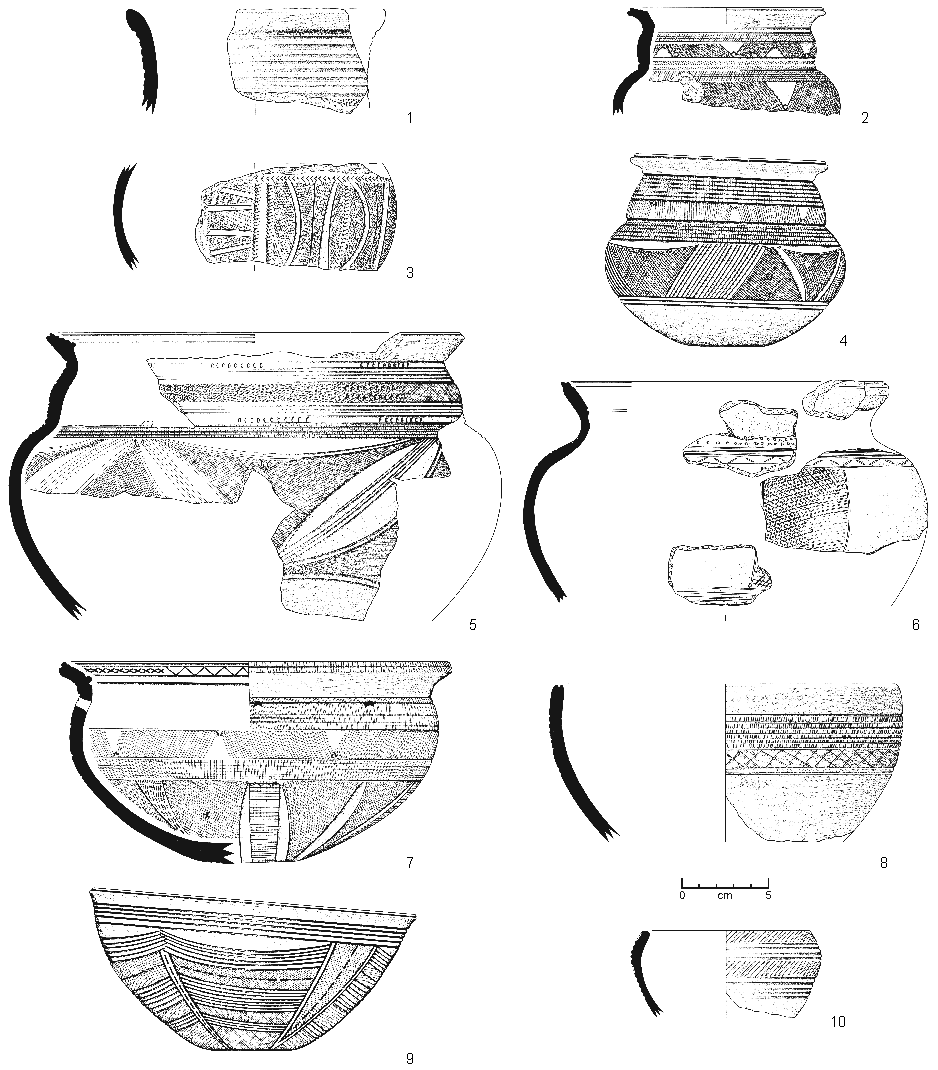
\includegraphics[width=\textwidth]{fig/BTM-Typen.pdf}
	\caption{Batalimo-Maluba-Gruppe: Typvertreter.\\1:~Taf.~11.1; 2:~Taf.~26.12; 3:~Taf.~11.2; 4:~Taf.~9.4; 5:~Taf.~26.9; 6:~Taf.~25.8; 7:~Taf.~9.3; 8:~Taf.~26.7; 9:~Taf.~9.1; 10:~Taf.~27.6.}
	\label{Fig-BatMLB-Typvertreter}
\end{figure*}

\paragraph{Formen}\hspace{-.5em}|\hspace{.5em}%
Das Formenspektrum der Batalimo-Maluba-Gruppe wird von leicht bauchigen Gefäßen des Typs~C2, flachen Gefäßen mit kurzem Rand vom Typ~E5 und rundbauchigen Schalen vom Typ~I2 bestimmt (Abb.~\ref{Fig-BatMLB-Typvertreter}). Die dominierende Gefäßform und quasi \textit{Leitform} der Batalimo-Maluba-Gruppe sind leicht bauchige Gefäße mit runder Schulter, kurzem kegel- oder zylinderförmigem Hals und einem meist kurz ausbiegendem Rand (Typ~C2; \ref{Fig-BatMLB-Typvertreter}.2, 4--5; \textsc{De Bayle des Hermens} 1975: Taf.~34).\footnote{Die beschriebene Gefäßform wurde in der ursprünglichen Veröffentlichung des Fundmaterials aus Batalimo als Typ P1 beziehungsweise P2 definiert \parencites[Taf.~33--34]{deBayledesHermens.1975}[Umzeichnung bei][135 Abb.~5.1]{Eggert.1987c}. Der Typ P1 umfasst Gefäße mit leicht einbiegendem konvexem Hals, während der Typ P2 Formen mit einem geraden bis leicht ausbiegenden konvexen Hals beschreibt (\textsc{De Bayle des Hermens} 1975: Taf.~34; Abb.~\ref{Fig-BatMLB-Typvertreter}.2,4--5). Im Material aus dem nordwestlichen Kongobecken hat sich eine solche Unterscheidung als nicht diagnostisch erwiesen und rechtfertigte daher nicht die Definition entsprechender Untertypen.\label{ftn:BatalimoGefTypen}} Im Material wurden insgesamt 57~GE dieses Typs beobachtet, wobei nur in 27 Fällen die Form sicher angesprochen werden konnte. Bei 29 GE war eine zweifelsfreie Zuweisung nicht möglich und in einem Fall war die Abgrenzung zur Schalenform E5 aufgrund der vorliegenden Fragmente nicht sicher. Die Gefäße des Typs C2 zeigen in 41\,\% der Fälle einen gerillten, ausbiegenden, kurzen Rand vom Typ B1.1. Gerillte Randabschlüsse sind bei etwa 62\,\% der GE dieses Typs nachgewiesen. Die Ausgestaltung der Gefäßhälse beschränkt sich auf eine Vielzahl von Varianten von geraden oder leicht bis deutlich konvexen Kegel- (A1/A2) oder Zylinderhälsen (B1/B2). Ein Untertyp mit einer leicht ausbiegenden Halspartie ist bislang nur aus Batalimo am Lobaye bekannt \parencite[Taf.~33]{deBayledesHermens.1975}.\footnote{Nur in einem Fall wurde eine vergleichbare Version des Gefäßhalses (Typ C1/B1) beobachtet. Die Gefäßschulter des Gefäßes weist einen schmalen Absatz zwischen Hals- und Schulterpartie auf, während regelhaft runde beziehungsweise konvexe Schulterpartien auftreten. Siehe Anm.~\ref{ftn:BatalimoGefTypen}.} Auffallend ist, dass die Gefäße des Typs C2 der Batalimo-Maluba-Gruppe in sehr unterschiedlichen Größen auftreten. Sie reichen von sehr kleinen Gefäßen mit einem Mündungsdurchmesser von lediglich 11\,cm (Abb.~\ref{Fig-BatMLB-Typvertreter}.4) bis zu großen Varianten mit bis zu 42\,cm Mündungsdurchmesser (Abb.~\ref{Fig-BatMLB-Typvertreter}.5). Die Gefäßhöhe entspricht regelhaft in etwa dem maximalen Durchmesser, wodurch die Gefäßproportionen bei elf GE, an denen Mündungshöhe und maximaler Durchmesser ermittelt werden konnte, zwischen etwa 1 zu 1,1--1,3 liegen.

Neben der beschriebenen, charakteristischen Form C2 beinhaltet das Material der Batalimo-Maluba-Gruppe auch bauchige Gefäße mit kurzem Kegelhals vom Typ~D1. Das Fundgut umfasst lediglich drei GE dieses Typs (Taf.~5.7).

Zusätzlich zu diesen beiden geschlossenen Gefäßformen umfasst das Spektrum der Batalimo-Maluba-Gruppe auch zwei offene Schalenformen. Schalen mit flachem Standboden (B4) und leicht konvexem Gefäßkörper vom Typ I2 (Abb.~\ref{Fig-BatMLB-Typvertreter}.8--9) ließen sich nur schwer im Fundgut identifizieren. Die zweite Variante bilden Schalen vom Typ E5 mit einer leicht einbiegenden, kurzen Schulter und einem ausbiegenden Rand. Waren die oberen Teile des Gefäßes, insbesondere der Halsbereich, nicht erhalten, war eine Abgrenzung zur Gefäßform C2 teilweise schwierig. Die Schalen des Typs E5 weisen, wenn sich die Maße abnehmen ließen, hinsichtlich des Verhältnisses von maximalem Durchmesser zur Höhe der Gefäßmündung Proportionen von etwa 2:1 auf (siehe Abb.~\ref{Fig-BatMLB-Typvertreter}.7, Taf.~25.5).

Die beobachteten Ränder der Batalimo-Maluba-Keramik (98~GE) wiesen regelhaft einen gerillten Randabschluss auf (64\,\%; Abb.~\ref{Fig-BatMLB-Typvertreter}.2, 4--9). Bereits deutlich seltener ließen sich runde (20\,\%) sowie gerade abgestrichene Randabschlüsse (10\,\%) beobachten. Das Gros der Ränder bilden kurze, einfach ausbiegende Ränder des Typs B1.1 (60\,\%; Abb.~\ref{Fig-BatMLB-Typvertreter}.2, 4--5, 7), gefolgt von längeren, einfach ausbiegenden Formen (B1; 14\,\%; Abb.~\ref{Fig-BatMLB-Typvertreter}.6). Noch seltener ließen sich ausbiegende, leicht rundlich verdickte Ränder vom Typ B1.4 nachweisen (7\,\%; Taf.~26.8, 27.2, 27.5). 

Bei 14 GE konnte die Bodenform angesprochen werden. In acht Fällen ließ sich ein flacher Standboden vom Typ B4 identifizieren. Jeweils in zwei Fällen kamen Linsenböden (B2) sowie Flachböden mit deutlich einziehender Unterseite (B5) vor. An jeweils einer GE ließ sich ein abgesetzter Flachboden (B11) sowie ein innen aufgewölbter Flachboden (B12) nachweisen.

\begin{figure*}[tb]
	\noindent\begin{minipage}[b]{\columnwidth}
		\includegraphics[width=\columnwidth]{fig/BTM_14C.pdf}
	\end{minipage}\hfill
	\noindent\begin{minipage}[b]{\columnwidth}
		\captionof{figure}{Batalimo-Maluba-Gruppe: Kalibierung der \textsuperscript{14}C-Datierungen aus Batalimo am Lobaye und Maluba am Lua (Fpl.~230) \parencites[233]{Aumassip.1975}{deMaret.1985b}{Eggert.1987c}{Kote.1992}{Eggert.1993}{Zangato.2000}.\label{fig:BTM14C}}
	\end{minipage}
\end{figure*}

\begin{figure*}[p]
	\centering
	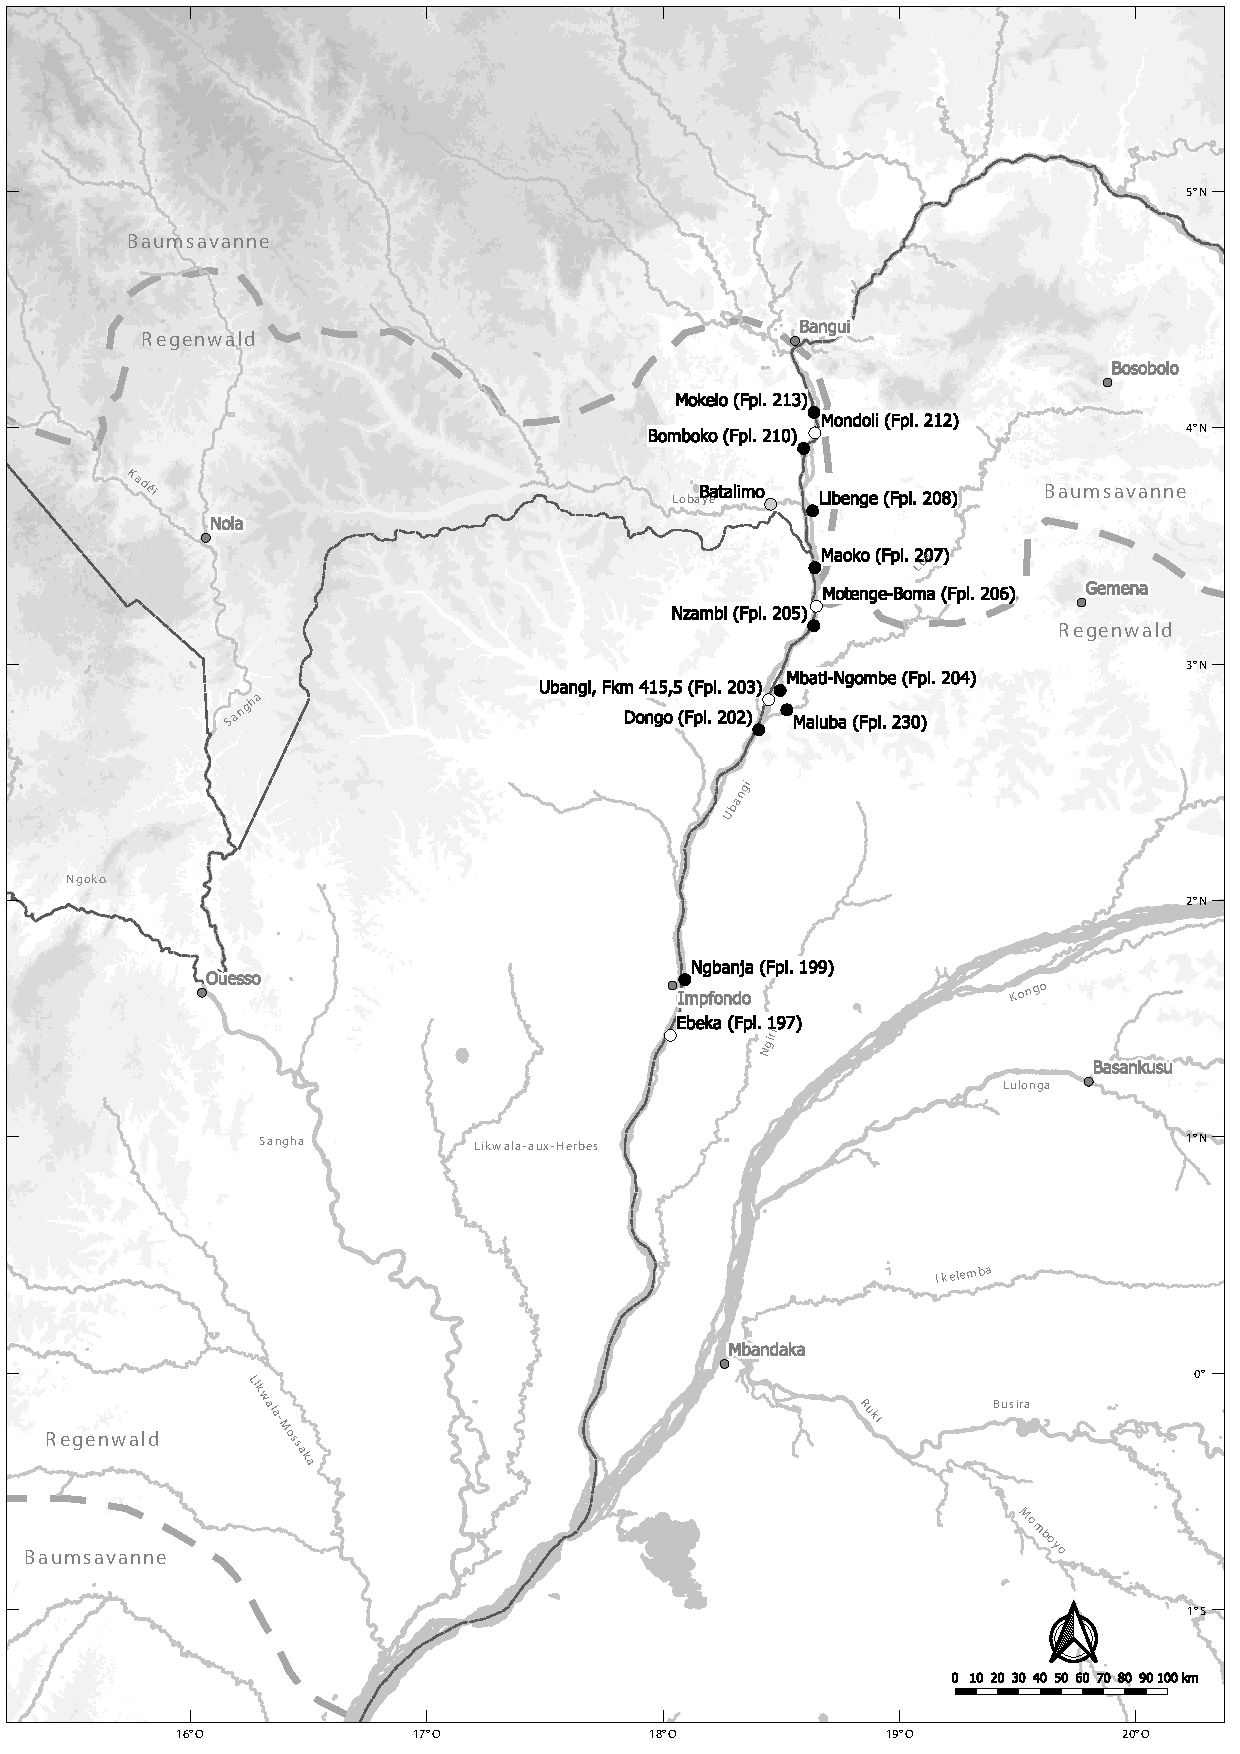
\includegraphics[width=\textwidth]{fig/BTM_Verbreitung.pdf}
	\caption{Batalimo-Maluba-Gruppe: Verbreitung \parencites[grau; nach][206]{deBayledesHermens.1975}[41\,f. Abb.~4]{Kote.1992}.}
	\label{fig:BTM-Verbreitung}
\end{figure*}

\paragraph{Verzierungen}\hspace{-.5em}|\hspace{.5em}%
Die Keramik der Batalimo-Maluba-Gruppe ist regelhaft verziert. Lediglich etwa 7\,\% aller GE weisen keine Verzierung auf. Im Mittel fanden sich an den GE drei unterschiedliche Verzierungselemente. Mit Blick auf die Verzierungszonen fällt auf, dass die Unterteile und Böden der Batalimo-Maluba-Keramik bis auf äußerst wenige Ausnahmen unverziert sind (Anlage~4.1). Auch die Außenseite der Ränder sind grundsätzlich frei von Verzierungen. Auf den Innenseiten finden sich hingegen regelhaft mit dem Randabschluss parallel verlaufende Rillenbündel (Tab.~\ref{tab:Verzierungselemente}: 02.1). Überdies wurden Verzierungen auf den Hals- und Schulterbereichen sowie dem Bauch der Gefäße aufgebracht. Lediglich knapp 7\,\% aller GE zeigen Verzierungen außerhalb dieser Zierzonen. Das mit Abstand häufigste Verzierungselement bilden horizontale Rillen (Tab.~\ref{tab:Verzierungselemente}: 02.1; 42\,\%). Ebenfalls lassen sich aus überkreuzenden Rillen gebildete \textit{Schachbrett}-Muster (Tab.~\ref{tab:Verzierungselemente}: 01.2; 7\,\%) und Rillen in Zickzack-Mustern (Tab.~\ref{tab:Verzierungselemente}: 01.6; 4\,\%), sowie diagonale (Tab.~\ref{tab:Verzierungselemente}: 02.3; 5\,\%) und gebogene Rillenbündel (Tab.~\ref{tab:Verzierungselemente}: 02.5; 4\,\%), häufig in Kombination miteinander, beobachten. Auffällig ist auch die Unterteilung von Gruppen von Verzierungselementen durch vertikale Rillen (Tab.~\ref{tab:Verzierungselemente}: 02.2; 4\,\%), was zu einer metopenartigen Strukturierung der verzierten Gefäßoberfläche führt. Des Weiteren zeigen die GE auch horizontale Bänder mit runden beziehungsweise leicht ovalen (Tab.~\ref{tab:Verzierungselemente}: 04.11; 4\,\%) oder diagonal gesetzten, kantigen Eindrücken (Tab.~\ref{tab:Verzierungselemente}: 04.12; 4\,\%). Diagonaler Kammeindruck lässt sich ebenfalls beobachten (Tab.~\ref{tab:Verzierungselemente}: 05.1; 4\,\%). Aufgrund des hohen Anteils an miteinander kombinierten Verzierungselementen hat keiner der vertreten Typen, mit Ausnahme der horizontalen Rillen, einen deutlichen Anteil. Zwar insgesamt seltener, aber ebenfalls für die Keramik der Batalimo-Maluba-Gruppe charakteristisch sind kleine, winkelige (Tab.~\ref{tab:Verzierungselemente}: 04.6; 3\,\%) oder Kreisaugen-Eindrücke (Tab.~\ref{tab:Verzierungselemente}: 04.7; 2\,\%). 

\paragraph{Datierung}\hspace{-.5em}|\hspace{.5em}%
Aus beiden 1985 in Maluba am Lua ausgegrabenen Gruben, die Keramik der Batalimo-Maluba-Gruppe enthielten (Kat.-Nr. 1--2), stammen jeweils zwei Radiokohlenstoffdatierungen. Während eine Datierung (KI-2445) eine sehr große Standardabweichung aufweist, ergeben alle Proben jedoch grundsätzlich einen konsistenten Datierungsansatz für die Stilgruppe. Ohne die weite Spanne des Datums KI-2445 weisen die Datierungen auf einen Zeitansatz vom 2. Jh.~v.~Chr bis in das 6. Jh. n.~Chr. (Abb.~\ref{fig:BTM14C}).

Eine Scherbe aus der 1968 in Batalimo am Lobaye erfassten \textit{Kulturschicht} -- Z\,I nach \textcite[117\,f. Tab.~10]{Kote.1992} -- wurde mittels Thermolumineszenzdatierung in das 1. Jh.~v.~Chr bis in das 10. Jh. n.~Chr. datiert \parencite[233; OxTL-154a-4]{Aumassip.1975}. Eine in das 3. Jh. v.~Chr. bis 7. Jh. n.~Chr. datierende Radiokohlenstoffprobe stammt aus der Sondage von Vidal (Bereich Z\,II nach \textsc{Koté} 1992: 117\,f. Tab.~10). Die Grabungen von \textsc{Koté} (ebd. 117\,f. Tab.~10) lieferten sechs weitere Radiokohlenstoffdatierungen für den Fundplatz Batalimo. Eine Probe aus Grabungsschnitt Z\,IV, der an die 1981 durch Vidal angelegten Sondage anschließt, datiert in das 1.--6.~Jh.~n.~Chr. (Bdy-304). Zwei Datierungen aus der in Schnitt Z\,III erfassten Grube decken aufgrund hoher Standardabweichungen einen Zeitraum vom 6. Jh. v.~Chr. bis in das 6. Jh. n.~Chr. ab \parencite[Bdy-301, Bdy-306;][120]{Kote.1992}. Die drei Radiokohlenstoffdatierungen aus der Grube in Schnitt Z\,VI liegen deutlich auseinander. Während eine Datierung aus dem oberen Bereich der Grube in das 6.--11.~Jh. n.~Chr. fällt (Bdy-465), datiert eine Probe von der Grubensohle in das 15.--20.~Jh. n.~Chr. (Bdy-462; ebd. 121). Worin die Ursache dieses auffällig jungen Alters liegen, kann basierend auf dem vorliegenden Bericht von \textsc{Koté} (ebd.) nicht mehr nachvollzogen werden. Eine Schneckenschale von der Sohle derselben Grube lieferte eine Datierungsspanne vom 1. Jh. v.~Chr. bis 5.~Jh. n.~Chr. (Bdy-581; ebd. 121). Ohne genaue Kenntnis und Zuordnung von Befunden, Funden und Datierungsproben, kann die in Schnitt Z\,VI erfasste Grube folglich nur unter starken Vorbehalten und lediglich mit Blick auf die Radiokohlenstoffdatierung Bdy-581 der Batalimo-Maluba-Gruppe zugerechnet werden.\footnote{Während sich dieses letzte Datum mit den aus Maluba stammenden Datierungsansätzen für Keramik der Batalimo-Maluba-Gruppe in Einklang bringen lässt, muss für die zweitälteste Datierung aus dem Befund schon die aus der ersten Grabung im Jahr 1967 stammende Thermolumineszenzdatierung (OxTL-154a-4), herangezogen werden. Zwischen dieser und der Datierung Bdy-465 ergibt sich eine Überlappung der auf 2-Sigma kalibrierten Alterspanne (Abb.~\ref{fig:BTM14C}). Das jüngste Datum liegt vollkommen außerhalb der bekannten Datierungsspanne. Siehe Anm.~\ref{ftn:Kote1992ZuordnungProblem}.}

Insgesamt stehen für die Batalimo-Maluba-Gruppe fünf sicher mit entsprechender Keramik assoziierte Datierungen zur Verfügung (Abb.~\ref{fig:BTM14C}: OxTL-154a-4, KI-2444, KI-2445, GrN-13584 und GrN-13585). Des Weiteren fallen fünf Radiokohlenstoffdatierungen aus den Grabungen von Vidal und \textcite{Kote.1992} in Batalimo in die Zeitspanne, die ohne Vorbehalte mit Batalimo-Maluba-Keramik in Zusammenhang steht (Abb.~\ref{fig:BTM14C}: Bdy-301, Bdy-306, Bdy-304 und Bdy-581 sowie Gif-5894). Da jedoch unklar ist, wie das zusammen mit diesen Proben angetroffene Fundgut aussieht, können diese nicht zweifelsfrei der Batalimo-Maluba-Gruppe zugerechnet werden. Auch handelt es sich bei allen Datierungen um konventionelle Messungen, die zudem häufig sehr hohe Standardabweichungen aufweisen. Zusammenfassend kann anhand der gegenwärtig vorliegenden Daten nur das 2. Jh. v.~Chr. bis 6. Jh. n.~Chr. als Zeitansatz für die Batalimo-Maluba-Keramik gelten (Abb.~\ref{fig:BTM14C}).

\paragraph{Verbreitung}\hspace{-.5em}|\hspace{.5em}%
Keramik  des Batalimo-Maluba-Stils findet sich in einem deutlich abgegrenzten Raum entlang dem Oberlauf des \mbox{Ubangi} sowie im Bereich der Mündung des Lua (Abb.~\ref{fig:BTM-Verbreitung}). Die nördliche Grenze der Verbreitung liegt etwas stromauf des \mbox{Ubangi}-Bogens bei Mokelo (Fpl.~213).\footnote{Auffällig ist die Nähe des Verbreitungsgebietes der Batalimo-Maluba-Keramik zur rezenten Nordgrenze des äquatorialen Regenwaldes (Abb.~\ref{fig:BTM-Verbreitung}). Nimmt man jedoch die von \textcite[7 Abb.~4]{Maley.2001} postulierte Grenze der Verbreitung des Regenwaldes im 1.~Jt. v.~Chr. als Grundlage, so liegt das Gros der Fundstellen außerhalb des Waldes. Erst zukünftige Untersuchungen zur Paläo-Umwelt dieses Raumes werden jedoch in der Lage sein, das ökologische Umfeld zur Zeit des Batalimo-Maluba-Stils zu ergründen (siehe Kap.~\ref{sec:Palaeoumwelt}).} Im Süden reicht die Hauptverbreitung bis in den Bereich südlich der Mündung des Lua. Vereinzelte Stücke finden sich auch weiter südlich, so zum Beispiel in Ebeka (Fpl.~197) und \mbox{Ngbanja} (Fpl.~199). Entlang des Lua fand sich lediglich in Maluba (Fpl.~230) Keramik des Batalimo-Maluba-Stils.\footnote{Zusammengenommen lagen von den drei ebenfalls am Lua gelegenen Fundplätzen Imboto (Fpl.~231), Ilawa (Fpl.~232) und Fulu-Kaba (Fpl.~233) lediglich 22 GE vor, die aufgrund starker Fragmentierung nur in fünf Fällen einer keramischen Stilgruppe zugerechnet werden konnten. Dabei handelte es sich ausschließlich um Vertreter der jüngeren Stilgruppen Dongo (Kap.~\ref{sec:DON-Gr}), Motenge-Boma (Fpl.~\ref{sec:MTB-Gr}) und Dama (Kap.~\ref{sec:DAM-Gr}).} Das am unteren Lobaye gelegene Batalimo \parencite{deBayledesHermens.1975} liegt in der nördlichen Hälfte des Verbreitungsgebietes.

Zusätzlich zu Batalimo am Lobaye \parencite{deBayledesHermens.1975} sowie den durch das \textit{River Reconnaissance Project} erschlossenen, hier vorgestellten Fundstellen, wird Keramik der Batalimo-Maluba-Gruppe noch von zwei weiteren Fundplätzen berichtet: In Ngo Tchoro, das 1,5\,km nördlich von Batalimo wohl ebenfalls nahe des Lobaye liegt, erbrachte ein 2009 angelegter Testschnitt Keramik, die jener der Batalimo-Maluba-Gruppe entsprechen soll \parencite{Ndanga.2010}. Von der am \mbox{Ubangi} gelegenen, aber nicht näher lokalisierbaren Fundstelle Mongo~II wird eine Grube mit geschliffenen Beilen, Batalimo-Maluba-Keramik sowie Belegen für Eisenverarbeitung berichtet \parencite{Ndanga.20120623}.\footnote{Gegenwärtig ist keines der beiden keramischen Inventare aufgearbeitet und veröffentlicht.}